%%%%%%%%%%%%%%%%%%%%%%%%%%%%%%%%%%%%%%%%%%%%%%%%%%%%%%%%%%%%%%%%%%%%%%%%%%%%%%%%
%2345678901234567890123456789012345678901234567890123456789012345678901234567890
%        1         2         3         4         5         6         7         8

\documentclass[letterpaper, 10 pt, conference]{ieeeconf}  % Comment this line out
                                                          % if you need a4paper
%\documentclass[a4paper, 10pt, conference]{ieeeconf}      % Use this line for a4
                                                          % paper

\IEEEoverridecommandlockouts                              % This command is only
                                                          % needed if you want to
                                                          % use the \thanks command
\overrideIEEEmargins
% See the \addtolength command later in the file to balance the column lengths
% on the last page of the document



% The following packages can be found on http:\\www.ctan.org
%\usepackage{graphics} % for pdf, bitmapped graphics files
%\usepackage{epsfig} % for postscript graphics files
%\usepackage{mathptmx} % assumes new font selection scheme installed
%\usepackage{times} % assumes new font selection scheme installed
%\usepackage{amsmath} % assumes amsmath package installed
%\usepackage{amssymb}  % assumes amsmath package installed

\title{\LARGE \bf
Are Olympian Swimmers Reaching Their Peak Performance?
}

%\author{ \parbox{3 in}{\centering Huibert Kwakernaak*
%         \thanks{*Use the $\backslash$thanks command to put information here}\\
%         Faculty of Electrical Engineering, Mathematics and Computer Science\\
%         University of Twente\\
%         7500 AE Enschede, The Netherlands\\
%         {\tt\small h.kwakernaak@autsubmit.com}}
%         \hspace*{ 0.5 in}
%         \parbox{3 in}{ \centering Pradeep Misra**
%         \thanks{**The footnote marks may be inserted manually}\\
%        Department of Electrical Engineering \\
%         Wright State University\\
%         Dayton, OH 45435, USA\\
%         {\tt\small pmisra@cs.wright.edu}}
%}
 
\author{Raymond Adams}

\usepackage[toc,page]{appendix}
\usepackage{appendix}
\usepackage{url}
\usepackage{hyperref}
\usepackage{graphicx}
\begin{document}



\maketitle
\thispagestyle{empty}
\pagestyle{empty}


%%%%%%%%%%%%%%%%%%%%%%%%%%%%%%%%%%%%%%%%%%%%%%%%%%%%%%%%%%%%%%%%%%%%%%%%%%%%%%%%
\begin{abstract}

This paper presents data that suggest that swimmers perform better at older ages than what most swimmers have been competing over the years of the sport. Many people suppose that as athletes age their performance will decline. However, research shows that this might not be completely true because the age at which some swimmers are breaking personal and world records is slowly increasing.  

\end{abstract}


%%%%%%%%%%%%%%%%%%%%%%%%%%%%%%%%%%%%%%%%%%%%%%%%%%%%%%%%%%%%%%%%%%%%%%%%%%%%%%%%
\section{INTRODUCTION}

Man began competitive swimming in Britain around 1830 however, the sport did not reach the Olympics until 1896. In the time past, more has been added and altered to the game. For instance, when Britain created the sport the only strokes they swam were freestyle and breaststroke. However, between now and then humans have added additional strokes to the sport such as, backstroke and butterfly.

In swimming, competitions are so competitive that the races usually come down to milliseconds. Swimming, like many individual sports, is hard to drop time off of an athletes personal best. However, athletes have managed to continuously achieve this difficult task. These athletes must be doing something in order to enhance their performance throughout each year. I swam competitively for 16 years and have competed in numerous state events; I have always assumed that the primary way to to increase your speed was through form and technique. Yet, current studies have suggested that this boost in swimmers speed might be a result of these athletes getting closer their peak performance age. Most people understand that as we become older our ability to perform at a high capacity decreases. However, the shape of the rate at which these athletes are increasing and decreasing their speed is built much like a curve where the peak of the curve is the athlete's peak performance. "In swimmers, the age-related decline in performance was reported to be influenced by the race distance and differed between women and men for short-distance pool-swimming" (Rust, pg 2). This piece of writing examines how women arrive at their peak performance faster than men. This seems to suggest that men do not reach their full potential until an older age than women especially in short distance races.  "In ultra-endurance swimming, peak swimming performance was achieved between 30 and 39 years for both men and women" (Rust, pg. 2). This data supports the allegation that Olympic swimmers times are improving due to them competing in these competitions at older ages. 

The first step I took in my research was to search for data on all the world records ever set for swimming. However, for the objective of this paper I chose to only collect information on 50 meter events. The reason I did this is because speed is illustrated through short distance races not long course events. After accumulating data for each stroke I then inserted the data into a table using excel. With this data alone the table presented valuable information but, I still
had to insert additional data so that I could wield specific graphs in Jupyter to better support my claim. The second step I took in my study was to discover articles that supported my claim. Each analyst did studies, supplied data, or supplied graphs that help determine whether swimmers are increasing their speed because of them swimming at an older age. 

Scientist suppose that professional swimmers are continuously breaking individual and world records at such an immense rate simply because these swimmers are competing closer to their peak performance age. "Peak performance" is when an person is able to perform at their max potential. Nearly all athletes reach this point regardless because most athletes peak at younger ages. However, unfortunately most male swimmers do not reach this peak because studies done by "Fairbrother (2007) reported that the peak swimming performance for 50 m freestyle was achieved at an older age in men" (Rust, pg. 2) but, the majority of male swimmers do not compete at this age. Nevertheless, male swimmers are starting to compete in these competitions at older ages each year. From the information that I have composed one can see that an increase in age is proportional with the increase in speed of a swimmer until a specific age. After that performance starts to decline.

\section{Literature Review}
The first article I came across, titled "Increase in the Age of Olympic Swimmers in Modern Times" written by Mazzilli, explains how research has shown an increase in age for long course and short course events for female and male athletes respectively competing in the Olympic games. ~\cite{mazzilli_2017}

The second article that I reviewed, titled  "The determinants of performance in master swimmers: an analysis of master world records" written by Zamparo, examines the age that swimmers reach there peak performance. ~\cite{zamparo_gatta_prampero_2012}

The third article, titled "The changes in age of peak swim speed for elite male and female Swiss freestyle swimmers between 1994 and 2012" written by Christoph Alexander Rust, speaks on the "changes in the age of peak freestyle swimming performance from 50 to 1,500 m for both elite female and male swimmers over time in recent years". Rust discovered that female swimmers reach their peak a lot quicker than men. A representation of this is shown later in figure 3. Rust's results were essential to help proving my claim true. His data showed that "age was positively associated with swimming speed for 50 - 800 m freestyle, but negatively for the 1,500 m freestyle. This suggests that athletes would be faster at higher ages with the exception of the 1,500 m freestyle." (Rust, pg. 7). This discovery causes one to wonder if an increase in age of a swimmer will lead to a faster times. ~\cite{rüst_knechtle_rosemann_lepers_2013} 

The fourth article that I reviewed, titled "Peak performance and age: An examination in peak performance in sports" written by K. Anders Ericsson, objective was to find athletes who were interested in attaining their peak performance. Ericsonn was interested in discovering the underlining biology that allows a person to reach their max potential. One of his goals was to determine whether the amount of time an athlete spends own his or her craft effects their peak performance. This research is crucial to my own because it implies that peak performance is not just automatically attained, it is something that you must work for. ~\cite{ericsson}

The fifth article that I reviewed, titled "Peak Performance and Age Among Superathletes: Track and Field, Swimming, Baseball, Tennis, and Golf" written by Richard Schulz and Christine Curnow, seeks to determine the age at which athletes in certain sports reach their peak performance. Schulz and Curnow discuss how the peak performance age for swimming is much higher than most sports. This is why I believe swimmers should continue swimming until their mid thirties in order to perform at their climax. ~\cite{schulz_curnow_1988}

The sixth article that I found, titled "Cheers vs. Jeers: Effects of Audience Feedback on Individual Athletic Performance" was written by L. Kimberly Epting, Kristen. Riggs, Joseph D. Knowles, and John J. Hanky. This journal discusses the effects that an audiences support (cheering) has on athletes in sports. The authors noted that "there are few experimental investigations of whether distinctive types of audience feedback have differential effects on athletes’ performance of particular sports skills." (Epting, pg. 299). However, their research showed that certain athletes thrive off audiences exuberance while others were not affected at all. It also showed that an audiences' jeer negatively hurt the performance for certain athletes. The reason that I reviewed this article is because I am curious on why swimmers do not stay in the sport for as long as most athletes do in other sports. I believe it may have something to do with inability of the audience being able to affect the swimmers through cheering. ~\cite{epting_riggs_knowles_hanky_2011}

The seventh article that I looked into, titled "Relationships among swimming performance, body composition and somatotype in competitive collegiate swimmers" was written by William A. Siders, Henry C. Lukaski, and William W. Bolonchuk. This article studied the connection amidst "swimming performance, body composition and somatotype" (Siders, pg. 166). ~\cite{a_c_w_1993}

The eighth article that I read, titled "Performance enhancement in swimming: The effect of mental training with biofeedback" was written by Bar-Eli M. and Blumenstein B. In this review, the comparison among "mental training with biofeedback and swimmers' performance was investigated." (Blumenstein). ~\cite{bar-eli_blumenstein_2004}

The ninth article that I read, titled "Physiological, biomechanical and anthropometrical predictors of sprint swimming performance in adolescent swimmers" was written by Priit Purge and other scholars. The goal of this study was to examine the connection the 100 meter freestyle performance "and relevant biomechanical, anthropometrical and physiological parameters in male adolescent swimmers." (Purge). ~\cite{e_j_p_r_k_kl_fa_t_2010}

The tenth article that I read, titled "Change of the age and performance of swimmers across World Championships and Olympic Games finals from 1992 to 2013 – a cross-sectional data analysis", was written by Stefan Koenig, Fabio Valeri, Stefanie Wild, Thomas Johannes Rosemann, Christoph Alexander Rust, and Beat Knechtle. The purpose of this article was to examine the difference in the age and performance of swimmers in the World Championships from 1994 to 2013 and Olympic Games from 1992 to 2012 in all events. These authors determined that in the last 20 years the top swimmers have increased in age and speed. This article helps show that it is very likely that the cause of the increase in performance of swimmers is due to them competing closer to their peak performance age. ~\cite{könig_valeri_wild_rosemann_rüst_knechtle_2014}

\section{Methods}
All of the data I collected came solely from Wikipedia and Exploratory. I first found a Wikipedia article that displayed the world record progression for each event. However, since I am only concerned with short distance races I only took data for 50 meter events. Therefore, I gathered data for the 50m freestyle, 50m breaststroke, 50m backstroke, and 50m butterfly. After I read through my piece of writing I recognized that the peak performance is not the same for men and women thus, I decided to gather information on both genders. Next I found a data set on Exploratory that displays the average age for male and female Olympic sports. I am using this data to show that the average age of swimmers is much younger than most athletes in different sports. Yet, the peak performance age for swimmers is much higher than other athletes. Assembling the data from both sites was a rather tedious task. First I copied each data entry to separate empty excel sheets. Then I decided to add new columns of my own from the data I collected from Wikipedia such as: Gender, Date, Stroke, and Age. This process took a very long time because I was forced to manually enter each data value into excel. I individually put data into 128 rows 4 times. However, only five of the ten rows in the data table were used to create the visualizations required to prove my claim valid. However, I will still explain every column so that as the reader you will have a firm grasp of the data in Figure 1. \url{https://en.wikipedia.org/wiki/World_record_progression_50_metres_freestyle} 
\begin{figure}
    \centering
    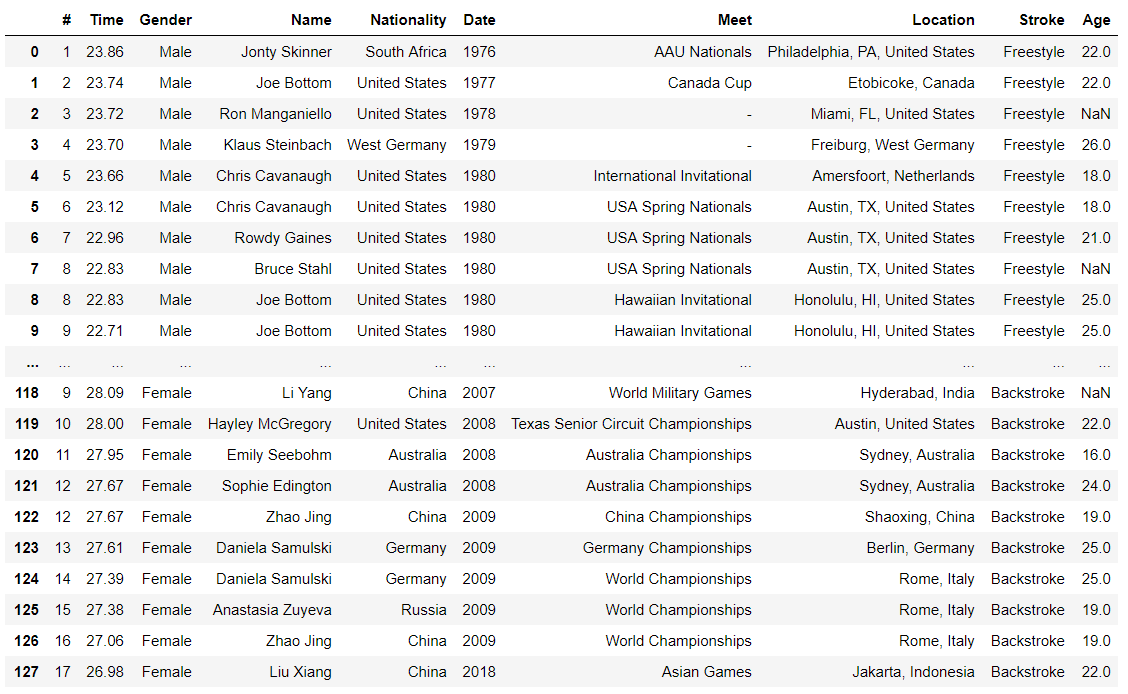
\includegraphics[width=8.5cm, height=7.5cm]{Data_Table}
    \caption{Table 1: World Record Progression}
    \label{Fig 1}
\end{figure}

%\begin{center}
 %   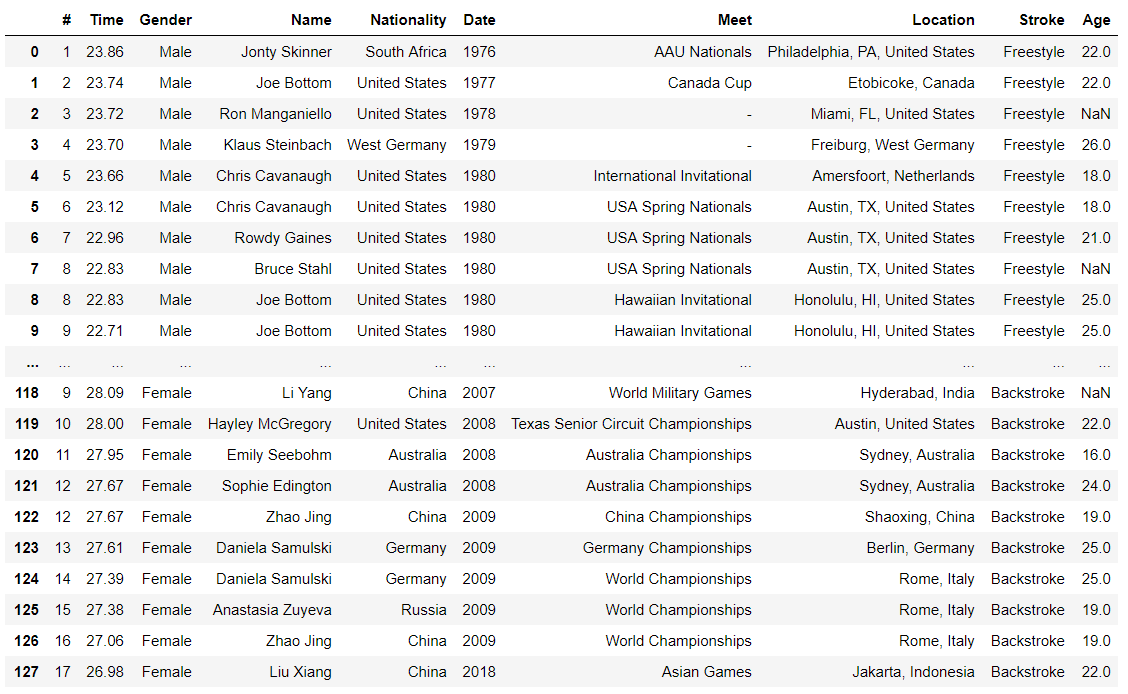
\includegraphics[width=8.5cm, height=7.5cm]{Data_Table}
  %  \caption{Table 1: WRP}
   % \label{fig: World Record Progression}
%\end{center}

 \begin{enumerate}
	\item  "\#" lists the every world record ever set in order for swimming in all 50 meter events.
    \item "Time" lists the world record time set by the swimmers' for a specific race.
    \item "Gender" lists the gender of each swimmer so that a comparison could be made between the two.
    \item "Name" lists the name of the athlete.
    \item "Nationality" lists the origin  of the swimmer.
    \item "Date" lists the year that the record was set.
    \item "Meet" lists the name of the meet. 
    \item "Location" lists the region where the race took place.
    \item "Stroke" lists the stroke of the race.
    \item "Age" lists the age of the swimmer at the time of the race. 
\end{enumerate}

\begin{figure}
    \centering
    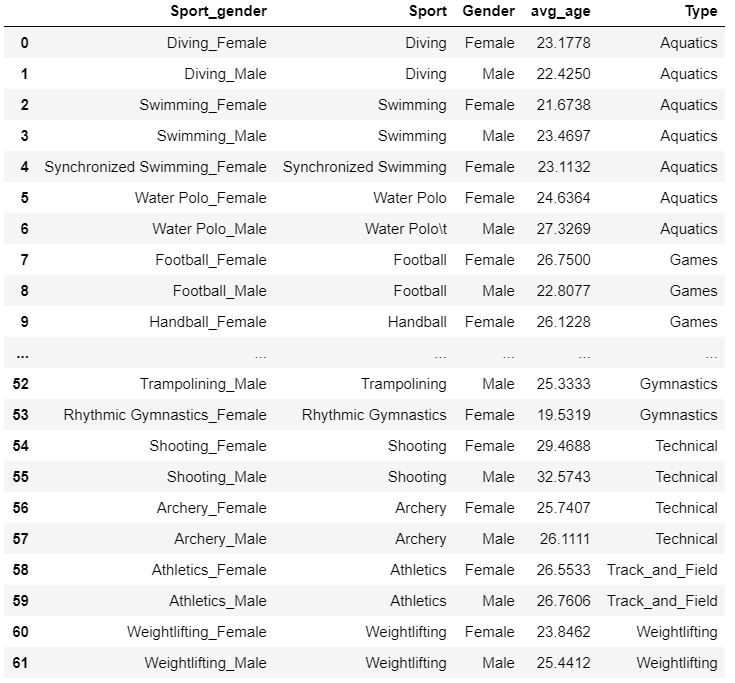
\includegraphics[width=8.5cm, height=7.5cm]{Avg_Age_of_Olympic_Athletes}
    \caption{Table 2: Avg Age of Olympic Athletes (London 2012)}
    \label{Fig 2}
\end{figure}

 For my second data table the only column that I added was "Type". I made this column so that I could sort each sport into a specific category. Figure 2 displays the average age of Olympians in each sport: \url{https://exploratory.io/viz/hideaki/9946fe75a197?cb=1471413911800}
 
 %\begin{center}
  %  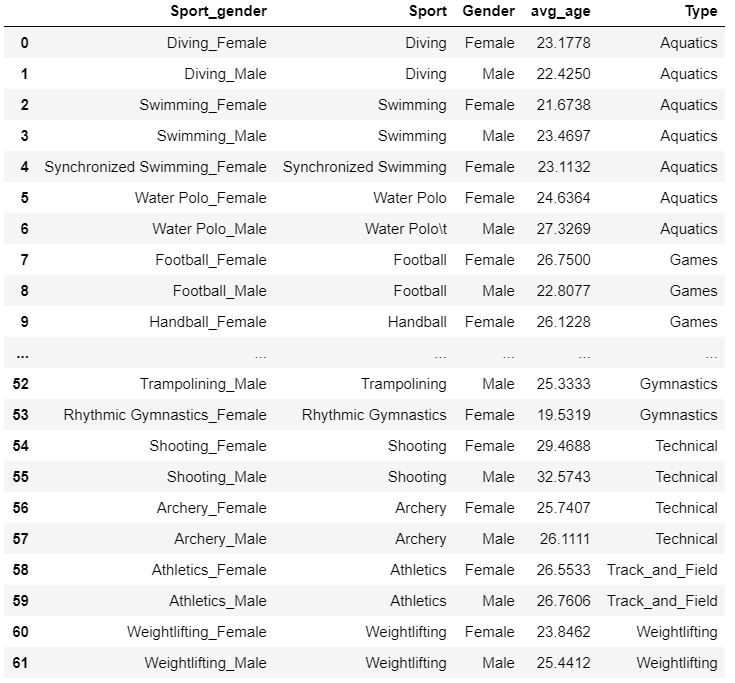
\includegraphics[width=8.5cm, height=7.5cm]{Avg_Age_of_Olympic_Athletes}
   % \caption{Table 2: }
    %\label{fig: Average Age of Olympic Athletes (London 2012)}
%\end{center}

 \begin{enumerate}
    \item "Sport\_gender" lists the name and gender of the sport separated by an underscore.
    \item "Sport" lists the name of the sport.
    \item "Gender" lists the sex of the athletes.
    \item "avg\_age" lists
\end{enumerate}

\section{Results}
I collected and manipulated my data from figure one to display the correlation between a swimmers' performance and age. The first graph that I created displays the age range and amount of Olympic record setters at that age for each stroke. Next I constructed a line graph that displays the rate at which male and female swimmers have progressed throughout the years of the sport. Finally, I made a linear regression plot that shows that the relationship between age and swimmers' time. 

\subsubsection{Age Range for World Record Holders}
\begin{figure}
    \centering
    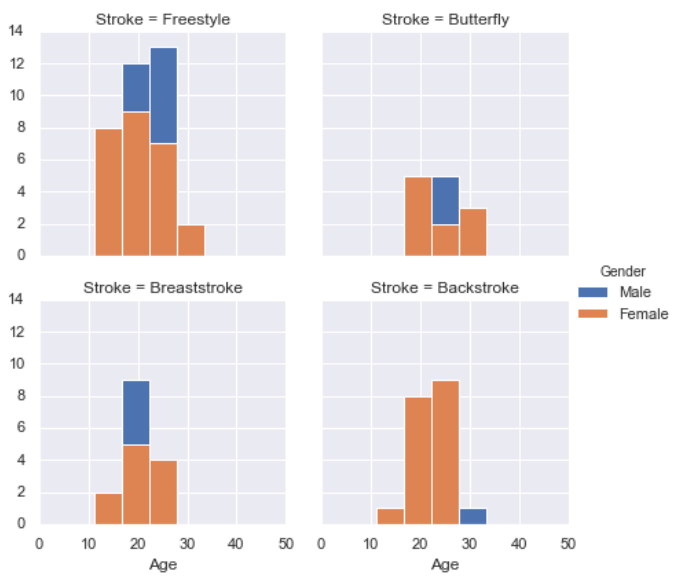
\includegraphics[width=8.5cm, height=7.5cm]{AverageAge}
    \caption{Avg Age of Olympic Athletes}
    \label{Fig 3}
\end{figure}

%\begin{center}
 %   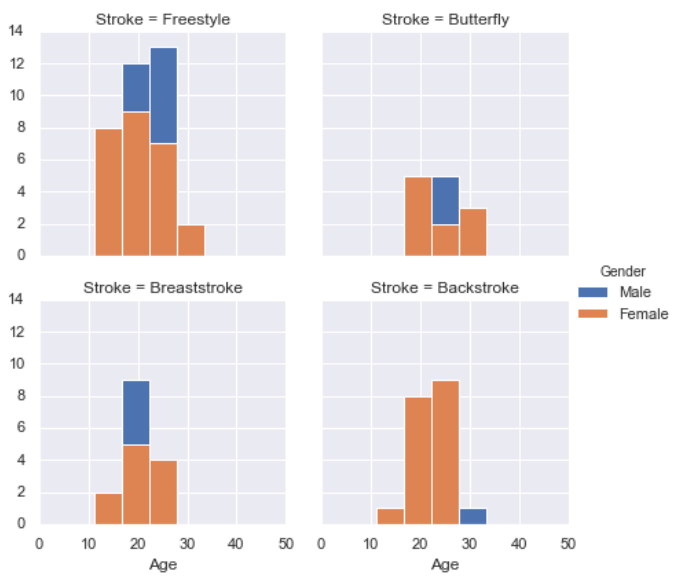
\includegraphics[width=8.5cm, height=7.5cm]{AverageAge}
  %  \caption{Figure 3: Avg Age of Olympic Athletes}
   % \label{Fig 3}
%\end{center}

In figure 3 I took the data that I gathered from figure 1 and plotted a small multiple histogram that displays the age range of Olympic World Record setters and the amount of athletes that fall in that same range. The goal of this chart is to show that the common age for male and female world record setters is early twenties. This shows that if my claims are true, almost all male and female swimmers are not competing at their full potential.

\subsubsection{Age Range for World Record Holders}
\begin{figure}
    \centering
    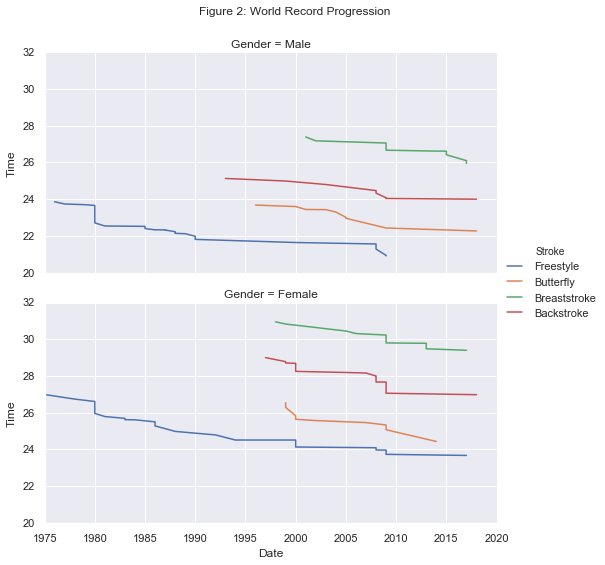
\includegraphics[width=8.5cm, height=7.5cm]{Rate_of_Progression.png}
    \caption{Rate of World Record Progression}
    \label{Fig 4}
\end{figure}
%\begin{center}
 %   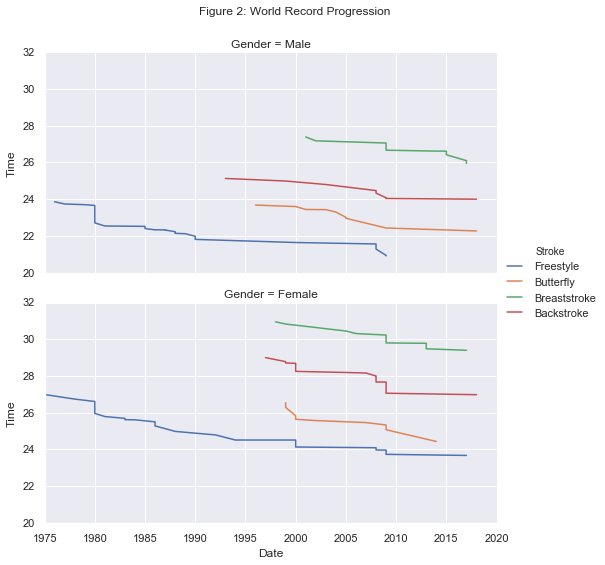
\includegraphics[width=8.5cm, height=7.5cm]{Rate_of_Progression.png}
  %  \caption{Figure 4: Age Range for Swimmers}
%\end{center}

In figure 4 I then took the same stats and plotted a time vs date line chart. This graph shows the rate at which these athletes times are improving over the years of the sport. The graph shows that swimmers are constantly getting faster throughout the years but at a slow rate.

\subsubsection{Average Age for Olympic Sports}
\begin{figure}
    \centering
    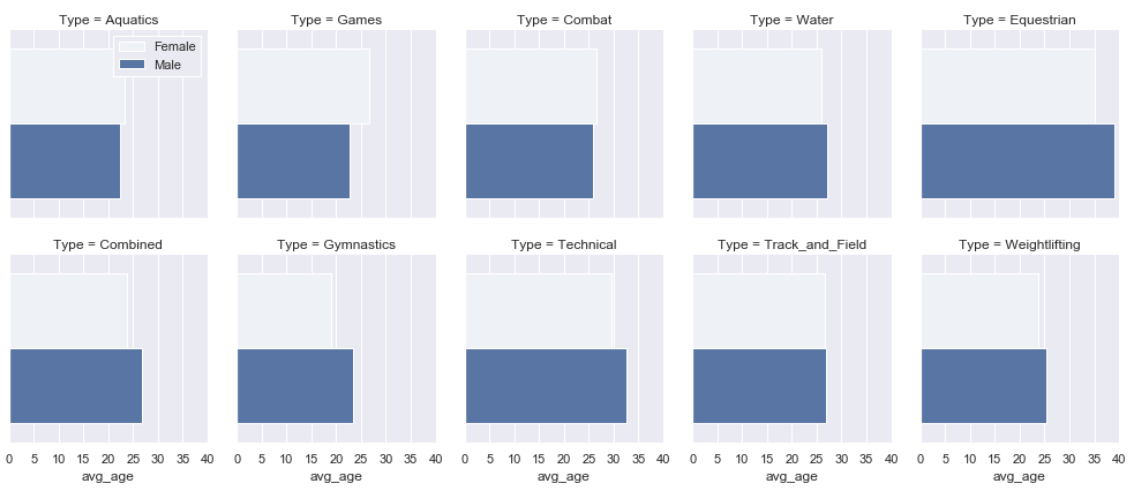
\includegraphics[width=8.5cm, height=7.5cm]{Avg_Age_for_Olympians.png}
    \caption{Avg Age for Olympic Sports}
    \label{Fig 5}
\end{figure}
%\begin{center}
  %  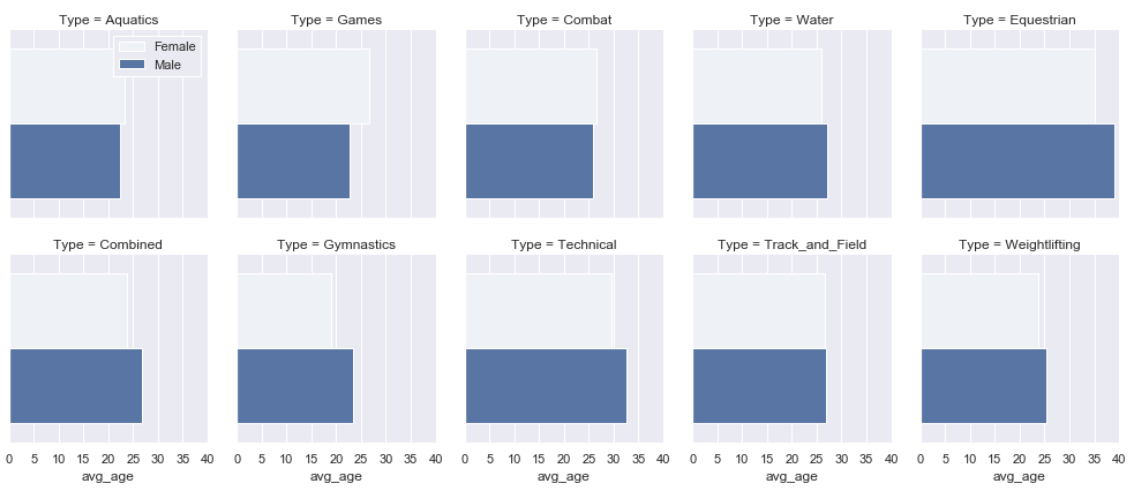
\includegraphics[width=8.5cm, height=7.5cm]{Avg_Age_for_Olympians.png}
 %   \caption{Figure 5: Avg Age for Olympic Sports}
%\end{center}

In figure 5 I took data from figure 2 and built a bar plot that displays the average age for female and male athletes by the type of sports in the Olympics. The purpose of this graph is to show that the average age for swimmers is very low compared to most other sports. I will later explain why I believe the average age for aquatic sports is so low.  

\subsubsection{Linear Regression}
\begin{figure}
    \centering
    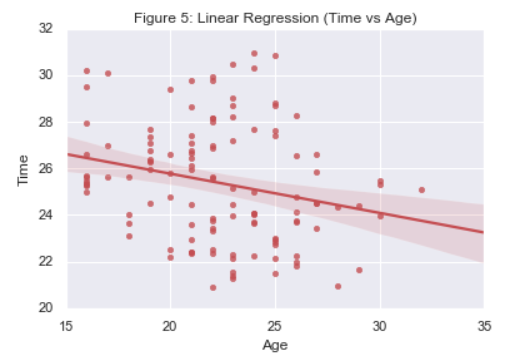
\includegraphics[width=8.5cm, height=7.5cm]{LinearReg.png}
    \caption{Linear Regression (Time vs Age)}
    \label{Fig 6}
\end{figure}

%\begin{center}
 %   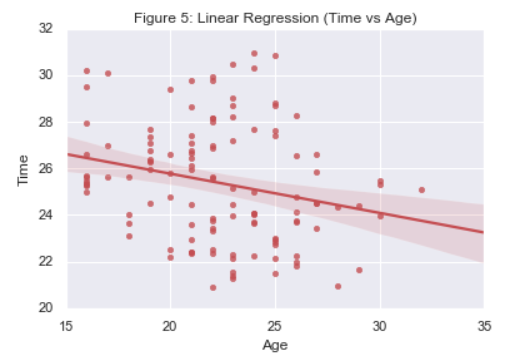
\includegraphics[width=8.5cm, height=7.5cm]{LinearReg.png}
  %  \caption{Linear Regression}
   % \label{Fig 6: Linear Regression (Time vs Age)}
%\end{center}

Finally in figure 6 I grabbed data from figure 1 again and created a linear regression that shows the comparison between age and speed of a swimmer. Through this graph you can see that age is positively correlated with time. This graph is the most important out of the rest because it suggest that as a swimmer ages his or her time actually decreases or gets faster. 


\section{Discussion}
In general, the results of this analysis suggest that as these Olympic swimmers increase in age they are steadily getting closer to their peak performance age thus, causing an increase in their speed. Figure 1 displays this growth. This graph shows that the elite swimmers, especially in freestyle, are presently swimming faster than swimmers in the 1900s due to an increase in the age of the athletes. Studies "showed in 2013 that the mean age of male swimmers was 21.1 years in 1984 but 25.8 in 2012, whereas the corresponding ages in women went from 18.9 to 21.6 years." (Mazzilli). This average age for male and female swimmers is shown in figure 5 under "Aquatics". Through studies and test scientists have determined that swimmers perform best in their mid 30s due to their peak performance age being so high. Unfortunately, as shown in figure 3 the majority of Olympic swimmers compete between the age of 20 and 25. As a result these athletes almost never perform at their peak. Lastly figure 6 displays the linear regression amongst speed and age. This graph implies that as a swimmer ages their times get faster. In conclusion these results are extremely important because they propose that a swimmer should keep competing until until their mid 30s in order to reach peak performance. 

\section{Conclusion}
To conclude, data has shown that there has been a growth in the average age of an Olympic Swimmer. This increase in age is believed to be the cause of the increase in speed of swimmers. Research has shown that the reasoning behind this correlation is due to swimmers peak performance being much higher than most athletes in other sports. In fact, swimmers do not reach their full potential until the age of "30 to 39" years old (Rust, pg. 2). This information is very substantial to these athletes because it implies that these athletes have an opportunity to perform for almost 10 extra years and still continue to set personal records. Unfortunately, I know that I am not the first person to discover this phenomenon. So, now the question is why aren't these athletes competing in the sport past their thirties? Through my research I came to an conclusion that swimmers usually do not compete past their mid twenties due to the lack of excitement that the competition creates. After swimming for 16 years myself I can say first hand that swimming is not a very enthusiastic sport. I believe that one of the reasons most athletes have a desire to continue the with their sport is due to the recognition and applause they receive during the competition. For example, in sports such as basketball and football, the athlete can constantly hear fans cheering or even jeering for them. This is what makes the games fun and exciting. However, when a swimmer is almost fully submerged in water all you hear is the sounds of arms and feet splashing and occasionally a muffled sound from the audience. Furthermore, the only time you can get a glimpse of where your competition is compared to you is when you go through your flip turn at the end of the pool. Thus, "Audience effects, then, may be very different than mere spectator effects." (Epting, pg. 202). I believe that these athletes grow tired of the sport and thus never reach their full potential. Nonetheless, the results from this study generates an important decision for modern day swimmers. These athletes must decide if it is worth staying in the sport for another 10+ years in order to reach their peak performance.   


\bibliographystyle{plain}
\bibliography{bibliography.bib}

\clearpage

\appendix
\subsection{Introduction}
\subsection{Literature Review}
\subsection{Methods}
\subsection{Results}
\subsection{Age Range for World Record Holders}
\subsection{Age Range for World Record Holders}
\subsection{Average Age for Olympic Sports}
\subsection{Linear Regression}
\subsection{Discussion}
\subsection{Conclusion}


\end{document}



